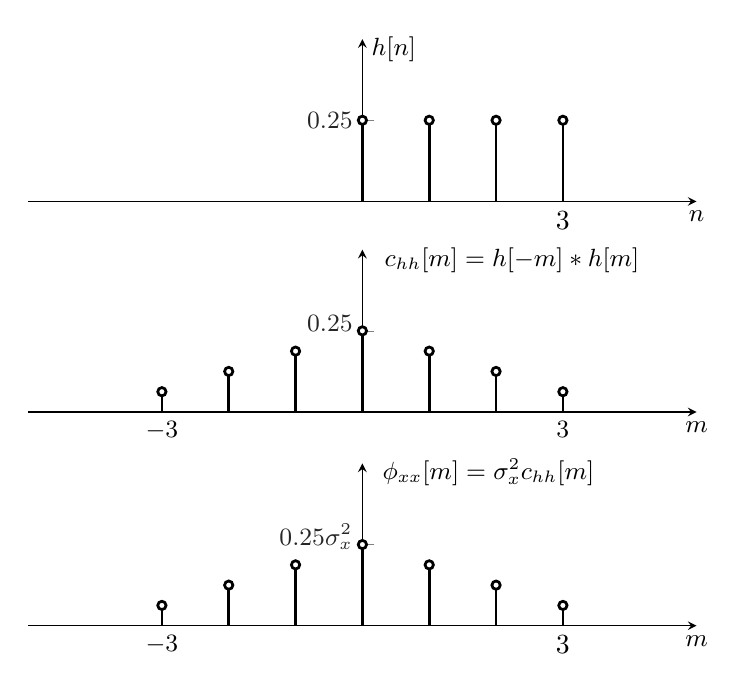
\begin{tikzpicture}
\begin{axis}[
	name=plot1,
	axis lines*=middle,
	enlargelimits = false,
	clip=false,
	scale only axis,
	width=0.7\textwidth,
	height=0.17\textwidth,
	ymin=0,
	ymax=0.5,
	xmin=-5,
	xmax=5,
	axis line style={->,>=stealth},
	xlabel={\small $n$},
	ylabel={\small $h[n]$},
	every axis x label/.style={
		at={(ticklabel* cs:1)},
		%xshift=0.2cm,
		anchor=north,
	},
	every axis y label/.style={
		at={(ticklabel* cs:0.8)},
		anchor=south,
		xshift=0.4cm,
	},
	%xtick=\empty,
	ytick={0.25},
	yticklabel={\small 0.25},
	xtick={0, 3},
	xticklabels={$0$, 3},
	every outer y axis line/.append style={white!15!black},
	every y tick label/.append style={font=\color{white!15!black}},
	legend style={draw=white!15!black,fill=white,legend cell align=left}]
	\addplot[ycomb, mark=*, fill=white, mark options={scale=0.75, fill=white}, line width=1pt, domain=0:3, samples=4] {0.25};
\end{axis}
\begin{axis}[
	name=plot2,
	at=(plot1.below south east), anchor=above north east,
	axis lines*=middle,
	enlargelimits = false,
	clip=false,
	scale only axis,
	width=0.7\textwidth,
	height=0.17\textwidth,
	ymin=0,
	ymax=0.5,
	xmin=-5,
	xmax=5,
	axis line style={->,>=stealth},
	xlabel={\small $m$},
	ylabel={\small $c_{hh}[m] = h[-m]\ast h[m]$},
	yticklabel style = {yshift=0.1cm},
	every axis x label/.style={
		at={(ticklabel* cs:1)},
		%xshift=0.2cm,
		anchor=north,
	},
	every axis y label/.style={
		at={(ticklabel* cs:0.8)},
		anchor=south,
		xshift=1.9cm,
	},
	ytick={0.25},
	yticklabel={\small 0.25},
	xtick={-3, 3},
	xticklabels={\small $-3$, \small 3},
	every outer y axis line/.append style={white!15!black},
	every y tick label/.append style={font=\color{white!15!black}},
	legend style={draw=white!15!black,fill=white,legend cell align=left}]
	\addplot[ycomb, mark=*, fill=white, mark options={scale=0.75, fill=white}, line width=1pt] coordinates {(-3, 0.0625)    (-2, 0.1250)    (-1, 0.1875)    (0, 0.2500)    (1, 0.1875)    (2, 0.1250)    (3, 0.0625)};
\end{axis}
\begin{axis}[
name=plot3,
at=(plot2.below south east), anchor=above north east,
axis lines*=middle,
enlargelimits = false,
clip=false,
scale only axis,
width=0.7\textwidth,
height=0.17\textwidth,
ymin=0,
ymax=0.5,
xmin=-5,
xmax=5,
axis line style={->,>=stealth},
xlabel={\small $m$},
yticklabel style = {yshift=0.1cm},
ylabel={\small $\phi_{xx}[m] = \sigma_x^2c_{hh}[m]$},
every axis x label/.style={
	at={(ticklabel* cs:1)},
	%xshift=0.2cm,
	anchor=north,
},
every axis y label/.style={
	at={(ticklabel* cs:0.8)},
	anchor=south,
	xshift=1.6cm,
},
ytick={0.25},
yticklabel={\small $0.25\sigma_x^2$},
xtick={-3, 3},
xticklabels={\small $-3$, 3},
every outer y axis line/.append style={white!15!black},
every y tick label/.append style={font=\color{white!15!black}},
legend style={draw=white!15!black,fill=white,legend cell align=left}]
\addplot[ycomb, mark=*, fill=white, mark options={scale=0.75, fill=white}, line width=1pt] coordinates {(-3, 0.0625)    (-2, 0.1250)    (-1, 0.1875)    (0, 0.2500)    (1, 0.1875)    (2, 0.1250)    (3, 0.0625)};
\end{axis}
\end{tikzpicture}
